\chapter{Instruction Set Architecture}

Processors understand bytes in groups of different sizes. The representation of
this grouping is different on various processors. When we're using this data, we
understand it fully as a group and don't break it up into different parts. We
consider these groups to be \textbf{words} (their term not mine). We would
naturally understand a group of bytes with the most significant byte written to
the left writing the next least significant byte to the right. For instance, a 4
byte word is shown below with the least significant byte being 0-indexed.

Which address is the most significant byte is called the endianness. If the
first addressable byte is the least significant byte this is little endian.
Otherwise, if the first addressable byte is the most significant byte this is
big endian.

\begin{center}
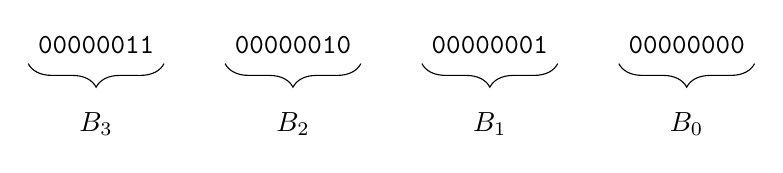
\begin{tikzpicture}
  \node (b3) {\ttfamily 00000011};
  \draw[decorate,decoration={amplitude=3mm,brace,mirror}]
    (b3.south west) -- (b3.south east);
  \node[below of=b3,anchor=center]{$B_3$};

  \node[right of=b3,node distance=2.5cm] (b2) {\ttfamily 00000010};
  \draw[decorate,decoration={amplitude=3mm,brace,mirror}]
    (b2.south west) -- (b2.south east);
  \node[below of=b2,anchor=center]{$B_2$};

  \node[right of=b2,node distance=2.5cm] (b1) {\ttfamily 00000001};
  \draw[decorate,decoration={amplitude=3mm,brace,mirror}]
    (b1.south west) -- (b1.south east);
  \node[below of=b1,anchor=center]{$B_1$};

  \node[right of=b1,node distance=2.5cm] (b0) {\ttfamily 00000000};
  \draw[decorate,decoration={amplitude=3mm,brace,mirror}]
    (b0.south west) -- (b0.south east);
  \node[below of=b0,anchor=center]{$B_0$};
\end{tikzpicture}
\end{center}

\section{x86-64}

We only discuss long mode (64-bit).
This is default mode for \texttt{x86\_64} processors.
There is 32-bit mode that is \texttt{x86} without any extensions (?) where
addresses are also 32-bit.
Another mode is \texttt{x32} which allows 32-bit addresses with the full
\texttt{x86\_64} instruction set.

\subsection{Encoding}

The main encoding is found in Intel's programming manual. This is a very
compressed version of the instruction encoding. All instructions start with a
prefix.

Legacy prefixes

Prefix group 2

$(64)_{16}$ FS segment override
$(65)_{16}$ GS segment override
$(2E)_{16}$ Branch not taken
$(3E)_{16}$ Branch taken

These are not used in long mode.
$(\texttt{2E})_{16}$ CS segment override
$(36)_{16}$ SS segment override
$(3E)_{16}$ DS segment override
$(26)_{16}$ ES segment override

Opcode with prefixes

ModR/M. Should be Mod.Reg.R/M

SIB

Displacement

Immediate

REX prefix, this prefix has 4 fields: W, R, X, B each are 1 bit. The first 4
bits of this prefix is $(\texttt{0100})_2$ or $(\texttt{4})_{16}$.

\subsection{Registers}

There are 16 ``general purpose'' 64-bit registers. How you address them is shown
below. All of these names are available in \texttt{x86\_64} mode. The rest of
them are there for legacy instructions.

Some registers are dedicated to the stack pointer, and source amnd destination
addresses.

% \begin{center}
% \begin{tikzpicture}
%   \node (r0) {\ttfamily Register 0};
%   \node[right of=r0, anchor=west] {\ttfamily rax};
% 
%   \node[below of=r0] (r1) {\ttfamily Register 1};
%   \node[right of=r1, anchor=west] {\ttfamily rcx};
% 
%   \node[below of=r1] (r2) {\ttfamily Register 2};
%   \node[right of=r2, anchor=west] {\ttfamily rdx};
% 
%   \node[below of=r2] (r3) {\ttfamily Register 3};
%   \node[right of=r3, anchor=west] {\ttfamily rbx};
% 
%   \node[below of=r3] (r4) {\ttfamily Register 4};
%   \node[right of=r4, anchor=west] {\ttfamily rsp};
% 
%   \node[below of=r4] (r5) {\ttfamily Register 5};
%   \node[right of=r5, anchor=west] {\ttfamily rbp};
% 
%   \node[below of=r5] (r6) {\ttfamily Register 6};
%   \node[right of=r6, anchor=west] {\ttfamily rsi};
% 
%   \node[below of=r6] (r7) {\ttfamily Register 7};
%   \node[right of=r7, anchor=west] {\ttfamily rdi};
% \end{tikzpicture}
% \end{center}

\subsection{Hello World}

\lstinputlisting{code/hello_world.asm}
%% \begin{listing}[H]
%%   \inputminted[frame=lines]{asm}{code/hello_world.asm}
%%   \caption{``Hello world'' program written in x86-64 assembly for Linux}
%%   \label{lst:hello-world-asm}
%% \end{listing}

Assuming the file is called ``\texttt{hello\_world.asm}'' we need to
compile to machine code using \texttt{nasm -f elf64
  hello\_world.asm}. This produces a file named
``\texttt{hello\_world.o}'' which is an object file (more later). To
produce an executable file that will run on the machine use the standard linker:
\texttt{ld hello\_world.o -o hello\_world}. This produces an
executable named ``\texttt{hello\_world}''. Running the program
using \texttt{./hello\_world} produces the output
``\texttt{Hello world!}''.

x86-64 has 16 general purpose registers: \texttt{rax},
\texttt{rbx}, \texttt{rcx}, \texttt{rdx},
\texttt{rbp}, \texttt{rsi}, \texttt{rdi},
\texttt{rsp}, \texttt{r8}, \texttt{r9},
\texttt{r10}, \texttt{r11}, \texttt{r12},
\texttt{r13}, \texttt{r14}, and \texttt{r15}. The
stack pointer is \texttt{rsp} and it is always(?) in use.

Note that the system call number goes in register \texttt{rax}. Note
that (on x86-64) the system call number for \texttt{write} is
\texttt{1} and for \texttt{exit\_group} is \texttt{231}. The arguments
to the system call go in registers according to the following table:

{\ttfamily\begin{tabular}{c c}
  \hline
  Index & Register \\
  \hline
  0 & \texttt{rdi} \\
  1 & \texttt{rsi} \\
  2 & \texttt{rdx} \\
  3 & \texttt{r10} \\
  4 & \texttt{r8} \\
  5 & \texttt{r9} \\
\end{tabular}}

In C, \texttt{rcx} is used instead of \texttt{r10} for the
argument at index 3. The kernel destroys registers in \texttt{rcx} and
\texttt{r11}. Registers \texttt{rbp}, \texttt{rbx},
\texttt{r12}, \texttt{r13}, \texttt{r14}, and
\texttt{r15} belong to the calling function and are untouched by the
kernel.
